\documentclass[lang=cn,newtx,10pt,scheme=chinese]{panpangis}

\usepackage{mdframed}
\renewcommand{\today}{\number\year 年 \number\month 月 \number\day 日}



\title{PanpanGIS文档}
\subtitle{PostgreSQL, PostGIS, SQLCarto, Apache, PHP, QT, QML}

\author{麓山老将,PcWang,隔壁老王}
\bioinfo{邮箱}{sqlcarto@163.com}
\institute{CSU.GIS.250 + 1}
\date{\today}
\version{1.0}


\extrainfo{
	支离东北风尘际,漂泊西南天地间。
	三峡楼台淹日月,五溪衣服共云山。\\ 
	羯胡事主终无赖,词客哀时且未还。
	庾信平生最萧瑟,暮年诗赋动江关。\\ 
	\hspace{8.5cm} ------ 杜甫(唐)
}

\setcounter{tocdepth}{3}

\logo{panpangis_logo2.png}
\cover{hometown02_small.jpg}

% 本文档命令
\usepackage{array}
\newcommand{\ccr}[1]{\makecell{{\color{#1}\rule{1cm}{1cm}}}}

% 修改标题页的橙色带
\definecolor{customcolor}{RGB}{32,178,170}
\colorlet{coverlinecolor}{customcolor}
\usepackage{cprotect}

\addbibresource[location=local]{reference.bib} % 参考文献,不要删除

\begin{document}

\maketitle
\frontmatter

\tableofcontents

\mainmatter

\chapter{缘起}

\section{还是干点啥吧}
去年冬日,麓山的树被冰雪压弯,折断不少枝叶,掉落在地。初春上午,孤独行走山间,绕过断枝残叶,
漫无目的爬向山顶。路边的小野花开得正旺,串串的淡黄,间或有几只蜜蜂起落其间。这种灌木开出的小花被父亲
叫做青叶子花,是初春重要的蜜源。脚下的残枝败叶与枝梢间的嫩芽正昭示着世间真理:旧的已去,新的正来。
当一个人在某个行当久了,成为资深,是否也正如这掉落的枝叶,在某个时间节点,无可奈地要随风去!?

外观落幕,内自落寞。离开吧!过去五年,这个声音一直耳边响着。从五楼搬到二楼,换到规律而boring的工作。
无人打扰,时间充足。Tong对我说,一个人一天接不到几个电话,接到的电话还是亲朋老友打过来的,说明没有希望了。



\chapter{Apache安装}

\section{Apache跨域设置}

如果web服务器的跨域参数设置不正确,在客户端为webassembly、服务端为https时,会出现
“a breakdown in protocol was detected (parsing error, invalid or unexpected responses, etc.)”
的错误。

修改apache.conf,添加如下设置:
\begin{minted}[obeytabs=true,tabsize=2,escapeinside=||,
	autogobble,frame=lines]{xml}
<Directory />
	AllowOverride none
	Require all denied
	|\bfseries{Header set Access-Control-Allow-Origin *}|
	|\bfseries{Header set Cross-Origin-Embedder-Policy 'require-corp'}|
	|\bfseries{Header set Cross-Origin-Opener-Policy 'same-origin'}|
</Directory>
\end{minted}



\chapter{Windows WSL(Ubuntu)子系统}

\section{WSL安装}

\section{将WSL迁移到非系统盘}

wsl 默认安装位置是C盘,众所周知C盘总是不够用的,所以才有了把 wsl 的系统迁移到其它位置的需求。在下列情况出现时需要将WSL从系统盘迁移(C)到非系统盘(D,E等):
\begin{itemize}
	\item 系统盘空间有限
	\item 数据库目录存在于WSL文件系统,但是预期数据库空间占用非常巨大
\end{itemize}


\subsection{查看所有分发版本}
\begin{lstlisting}[language=bash]
	wsl -l --all -v
\end{lstlisting}


\subsection{导出分发版为tar文件}
\begin{lstlisting}[language=bash]
wsl --export Ubuntu-20.04 D:\ubuntu20.04.tar
\end{lstlisting}


\subsection{注销当前分发版}
\begin{lstlisting}[language=bash]
wsl --unregister Ubuntu-20.04
\end{lstlisting}


\subsection{重新导入并安装分发版}
\begin{lstlisting}[language=bash]
wsl --import Ubuntu-20.04 D:\wsl\ubuntu D:\ubuntu20.04.tar --version 2
\end{lstlisting}


\subsection{设置默认登陆用户为安装时用户名}
\begin{lstlisting}[language=bash]
ubuntu2004 config --default-user Username
\end{lstlisting}


\chapter{使用msys2系统编译postgis/postgresql}

\section{安装msys2}
从\href{https://www.msys2.org/}{https://www.msys2.org/}网站下载msys安装包,双击安装msys2。

\begin{center}
	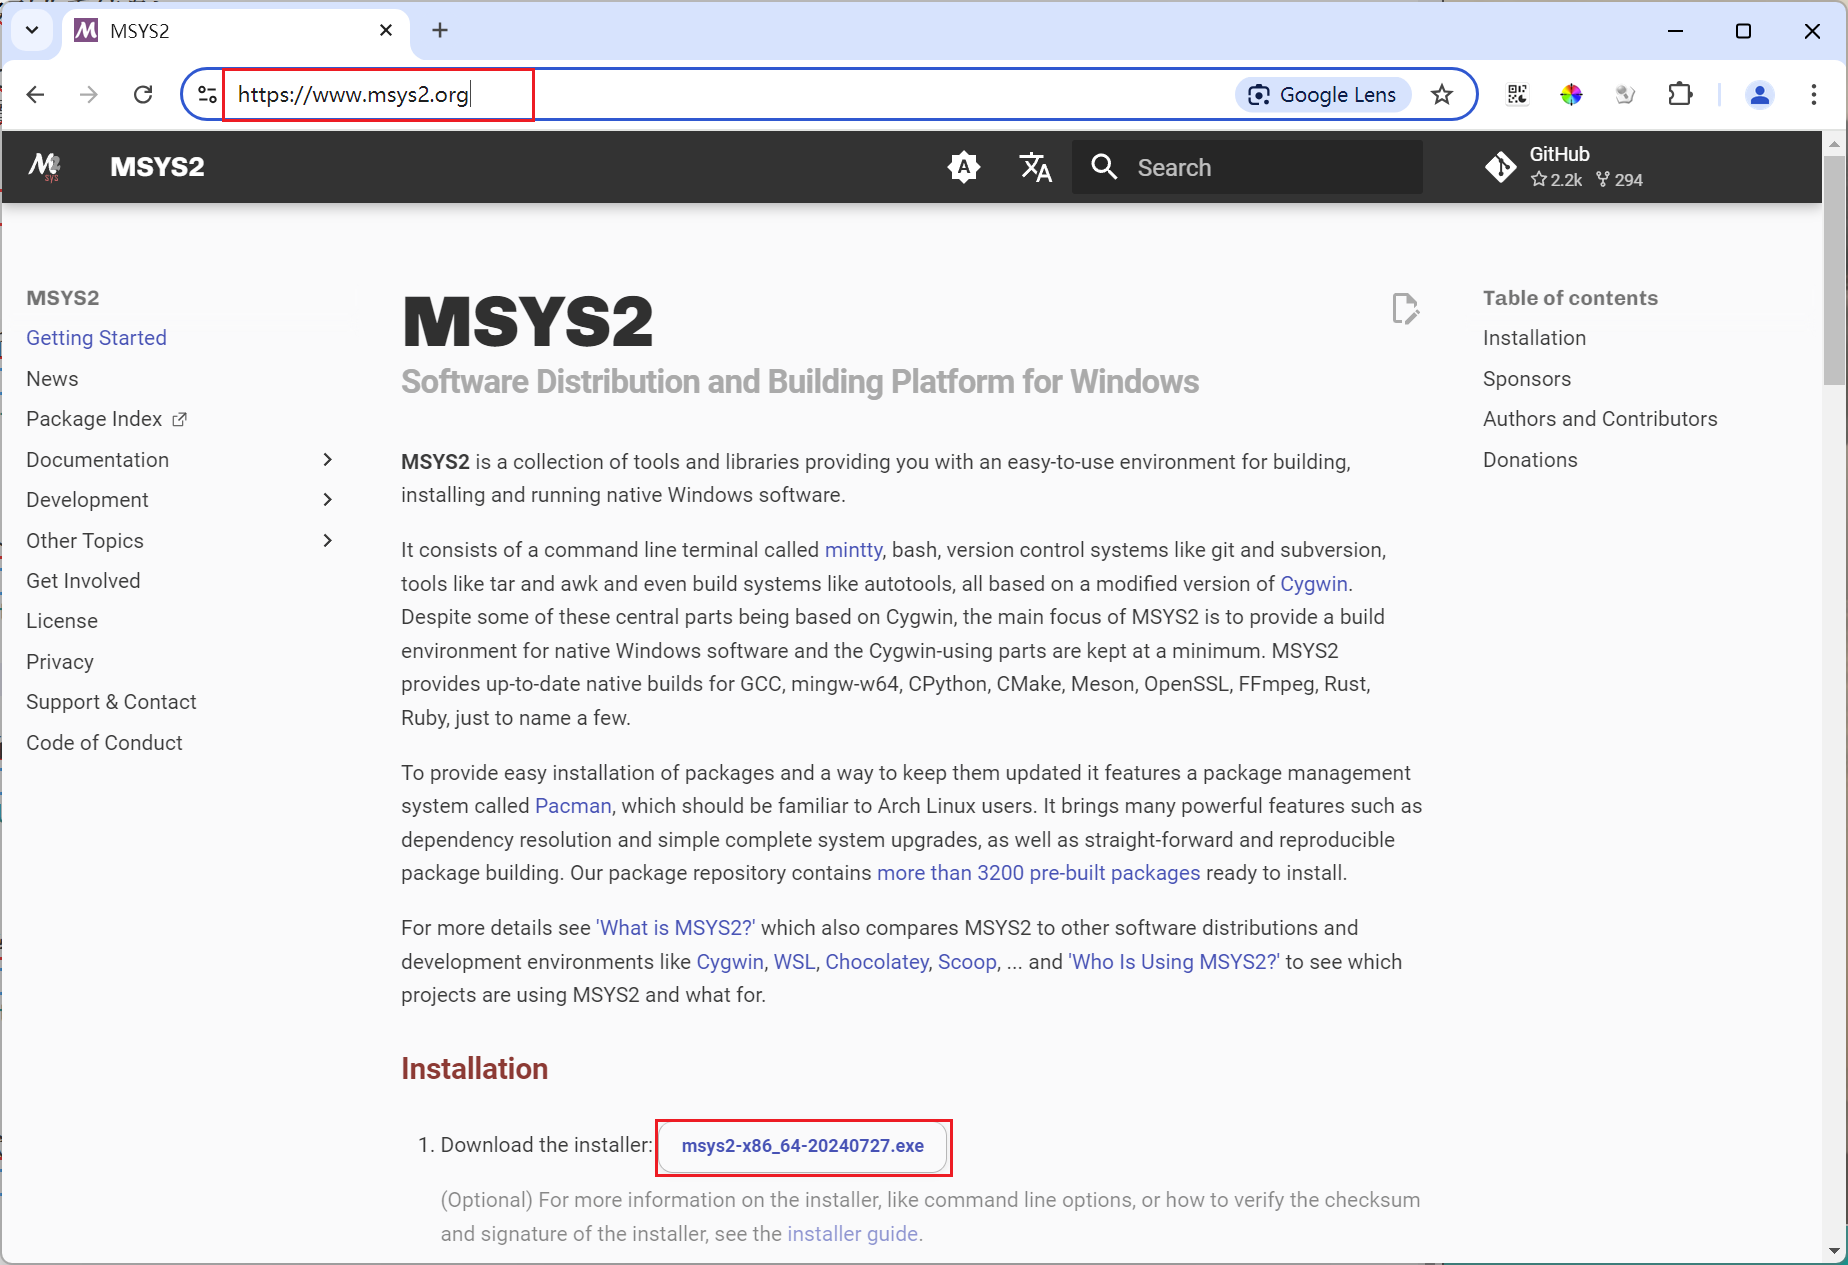
\includegraphics[width=0.8\textwidth]{03install/msys2_download.png}
\end{center}



\section{启动msys2 ucrt}
\begin{center}
	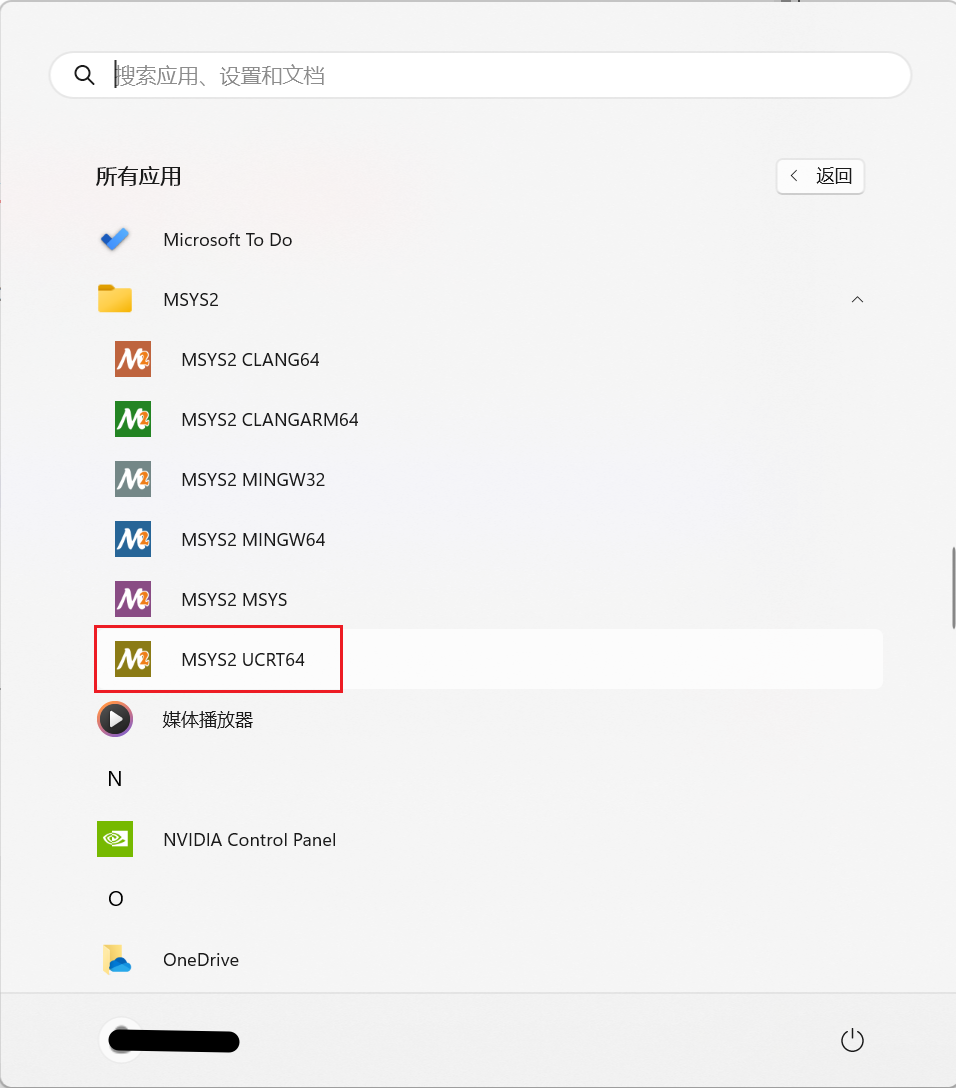
\includegraphics[width=0.5\textwidth]{03install/msys2_start.png}
\end{center}

\begin{center}
	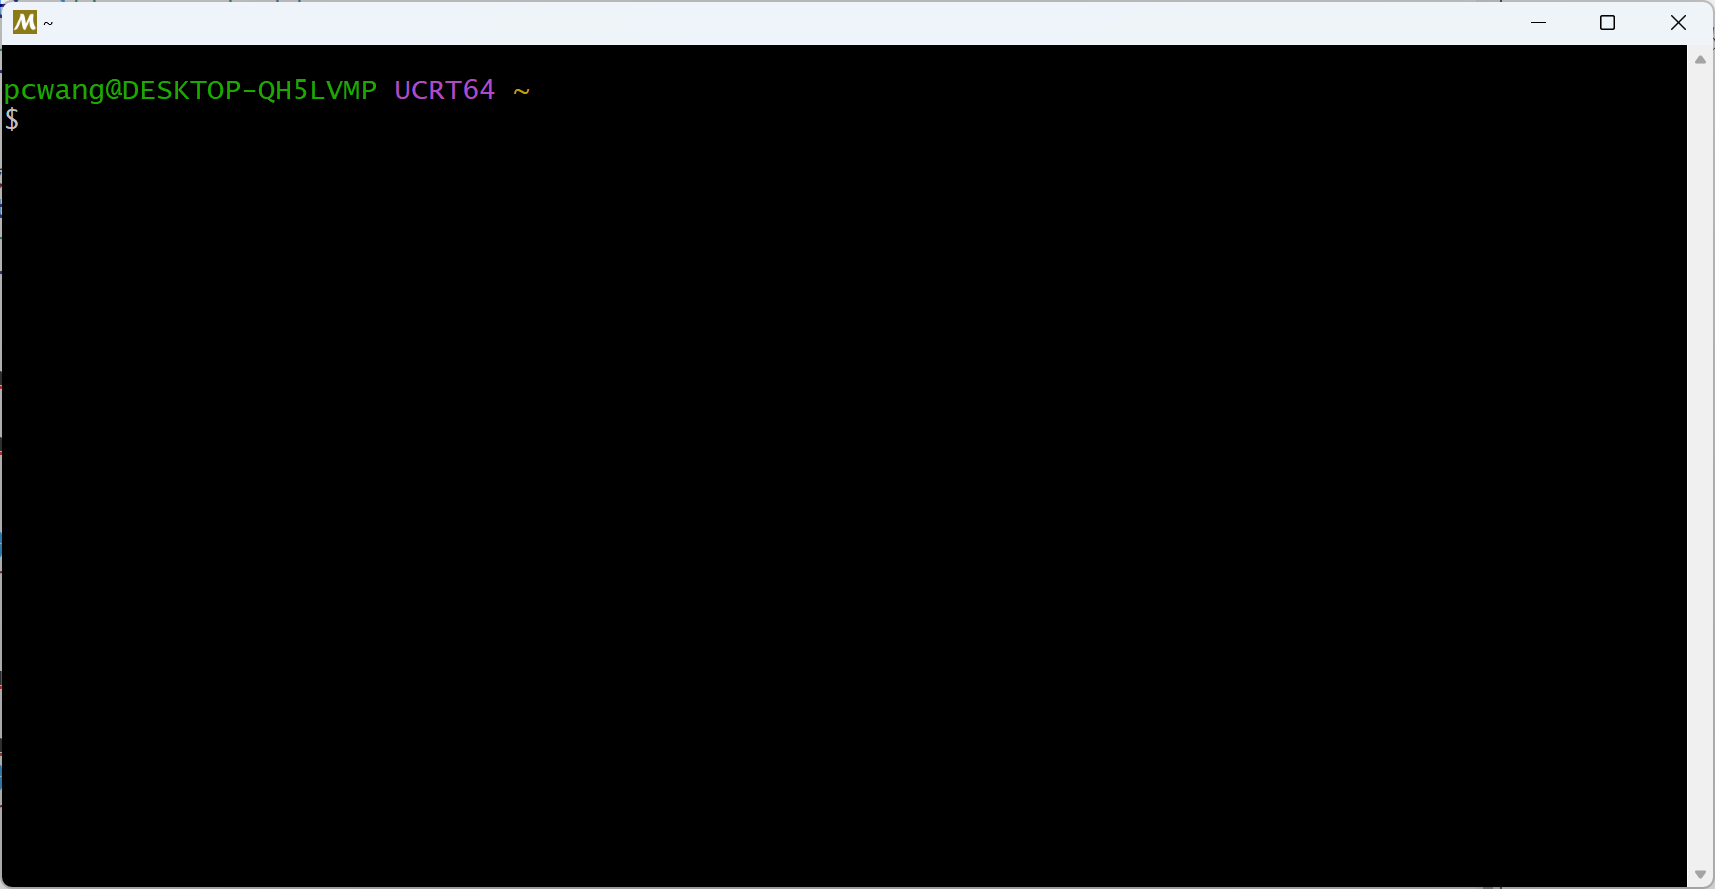
\includegraphics[width=0.8\textwidth]{03install/msys2_ucrt.png}
\end{center}

\section{安装ucrt编译工具链}

\subsection{查询工具链}

\begin{lstlisting}[language=bash]
	pacman -sS gcc | grep ucrt
\end{lstlisting}

\begin{center}
	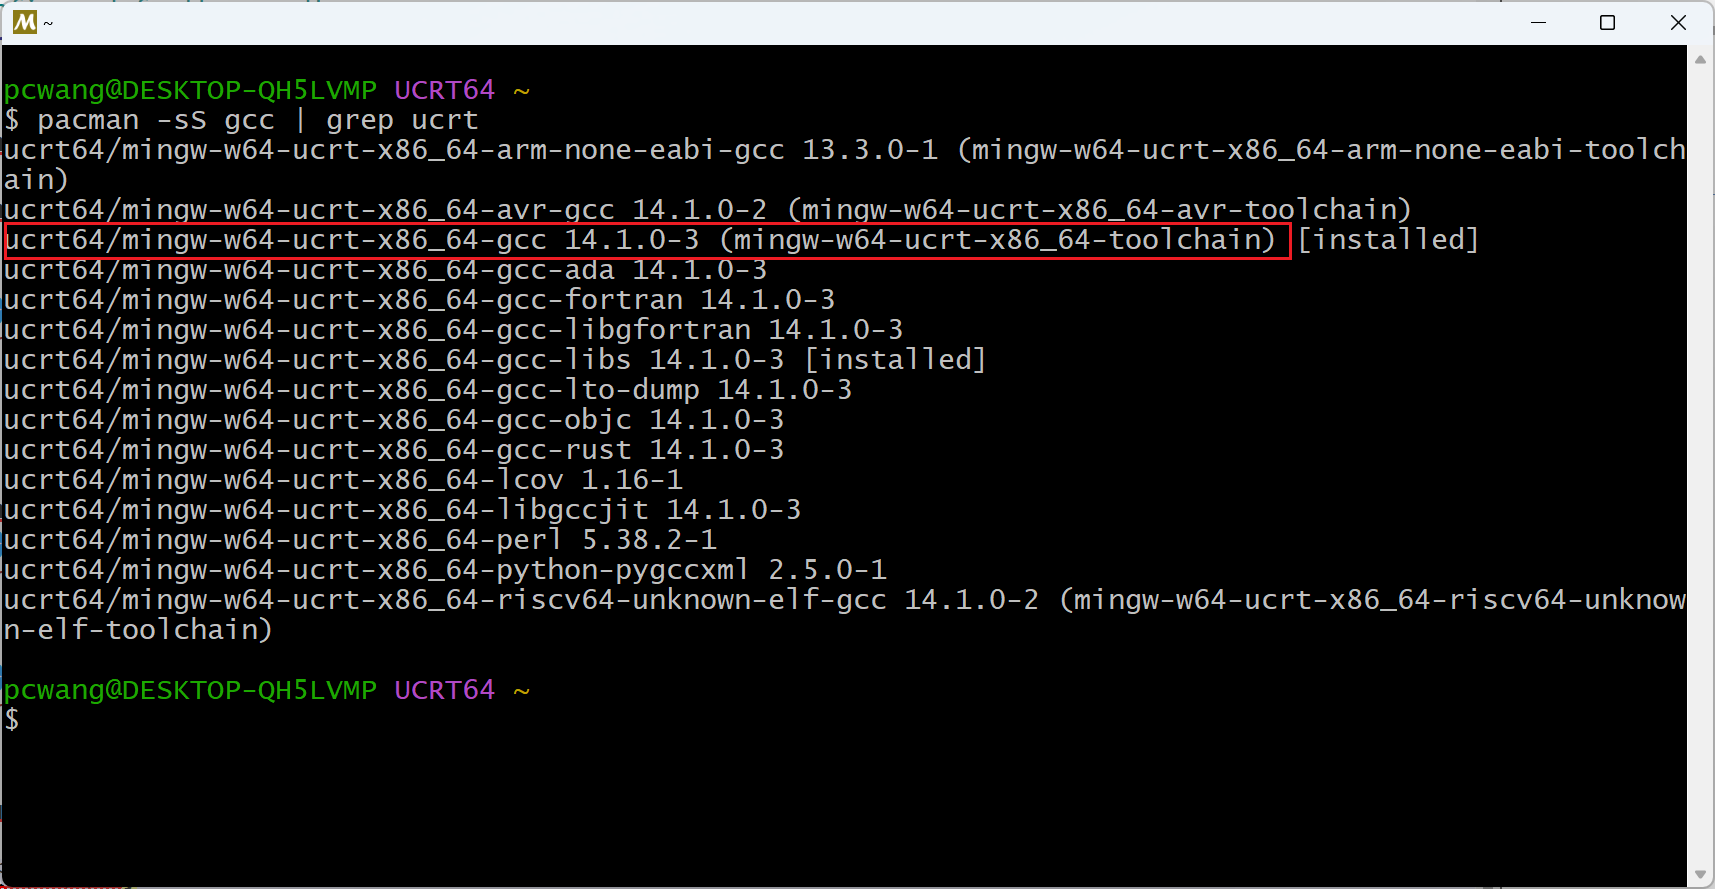
\includegraphics[width=0.8\textwidth]{03install/pacman_search_ucrt_gcc.png}
\end{center}

\subsection{安装工具链}

\begin{lstlisting}[language=bash]
	 pacman -S mingw-w64-ucrt-x86_64-toolchain
	 pacman -S ucrt64/mingw-w64-ucrt-x86_64-cmake 
	 pacman -S msys/make
\end{lstlisting}

\section{编译postgresql}
\subsection{设置环境变量}
编辑/etc/profile,在最末尾添加下列内容:
\begin{lstlisting}[backgroundcolor = \color{codebackground}, language=bash]
	export PGSQL=/usr/local/pgsql
	export PATH=$PGSQL/bin:$PGSQL/lib:$PATH
	export LD_LIBRARY_PATH=$PGSQL/lib:$LD_LIBRARY_PATH
	export PKG_CONFIG_PATH=$PKG_CONFIG_PATH:$PGSQL/lib/pkgconfig
\end{lstlisting}
重新启动msys2 ucrt命令行。

\subsection{安装支持库}

\begin{lstlisting}[backgroundcolor = \color{codebackground}, language=bash]
	# postgis利用cgal支持3D空间分析
	# sfcgal为cgal的c语言wrapper,只有c语言的库才能链接到postgresql
	pacman -S ucrt64/mingw-w64-ucrt-x86_64-sfcgal 
	
	# cairo为图形库,sqlcarto使用cairo进行二维地图绘制
	pacman -S ucrt64/mingw-w64-ucrt-x86_64-cairo 
	
	# libgeotiff为geotiff栅格文件的读写库,gdal需要
	pacman -S ucrt64/mingw-w64-ucrt-x86_64-libgeotiff 
	
	# netcdf读取大数据文件,地理空间栅格数据
	pacman -S ucrt64/mingw-w64-ucrt-x86_64-netcdf
	
	pacman -S ucrt64/mingw-w64-ucrt-x86_64-protobuf-c
\end{lstlisting}


\subsection{安装uuid}
\begin{lstlisting}[backgroundcolor = \color{codebackground}, language=bash]
	cd ~
	mkdir -p software/sdb
	cd software/sdb
	curl --output uuid-1.6.1.tar.gz ftp://ftp.ossp.org/pkg/lib/uuid/uuid-1.6.1.tar.gz
	tar -zvxf uuid-1.6.1.tar.gz
	cd uuid-1.6.1
\end{lstlisting}

使用编辑器打开shtool脚本文件,找到dsttmp变量赋值语句:
\begin{lstlisting}[backgroundcolor = \color{codebackground}, language=bash]
	...
	#   make a temp file name in the destination directory
	dsttmp=`echo $dst |\
		sed -e 's;[^/]*$;;' -e 's;\(.\)/$;\1;' -e 's;^$;.;' \
		-e "s;\$;/#INST@$$#;"`
	...
\end{lstlisting}

在后面添加一行,改成:

\begin{lstlisting}[backgroundcolor = \color{codebackground}, language=bash, escapeinside={(@*}{*@)}]
	...
	#   make a temp file name in the destination directory
	dsttmp=`echo $dst |\
		sed -e 's;[^/]*$;;' -e 's;\(.\)/$;\1;' -e 's;^$;.;' \
		-e "s;\$;/#INST@$$#;"`
	# 添加下面这一行
	(@*\textcolor[rgb]{0,0,1}{\textbf{dsttmp=\$dsttmp.exe}} *@)
	...
\end{lstlisting}

保存shtool文件,在控制台运行下列命令行,配置及安装uuid:

\begin{lstlisting}[backgroundcolor = \color{codebackground}, language=bash]
	./configure --prefix=$PGSQL
	make 
	make install
\end{lstlisting}

\subsection{安装postgresql}
\begin{lstlisting}[backgroundcolor = \color{codebackground}, language=bash, escapeinside={(@*}{*@)}]
	cd ~/software/sdb
	
	# 下载源代码
	# 注意curl命令使用的参数,此处模拟chrome来下载文件
	# 如直接使用:
	# curl 'https://ftp.postgresql.org/pub/source/v16.4/postgresql-16.4.tar.bz2' --output postgresql-16.4.tar.bz2
	# 则不能成功下载源码文件
	# 可以根据需要改变版本号来下载对应的版本的postgresql源码
	# curl 'https://ftp.postgresql.org/pub/source/v16.4/postgresql-16.4.tar.bz2' \
	#	-H 'Referer: https://www.postgresql.org/' \
	#	-H 'Upgrade-Insecure-Requests: 1' \
	#	-H 'User-Agent: Mozilla/5.0 (Windows NT 10.0; Win64; x64) AppleWebKit/537.36 (KHTML, like Gecko) Chrome/128.0.0.0 Safari/537.36' \
	#	-H 'sec-ch-ua: "Chromium";v="128", "Not;A=Brand";v="24", "Google Chrome";v="128"' \
	#	-H 'sec-ch-ua-mobile: ?0' \
	#	-H 'sec-ch-ua-platform: "Windows"' \
	#	--output postgresql-16.4.tar.bz2
	# 使用curl的-LJO 参数下载文件
	curl -LJO 'https://ftp.postgresql.org/pub/source/v16.4/postgresql-16.4.tar.bz2'
	
	tar -jvxf postgresql-16.4.tar.bz2
	cd postgresql-16.4
	# 由于uuid没有安装在/usr目录,而是安装在$PGSQL目录下,因此在配置时
	# 应该指定LDFLAGS和CPPFLAGS环境变量,否则会提示找不到uuid库
	LDFLAGS="-L$PGSQL/lib" CPPFLAGS="-I$PGSQL/include" ./configure --prefix=$PGSQL --with-ossp-uuid
	make
	make install
	
	# 编译postgresql的uuid扩展
	cd contrib/uuid
	make
	make install
\end{lstlisting}

\subsection{安装geos}
geos提供空间分析功能。
\begin{lstlisting}[backgroundcolor = \color{codebackground}, language=bash, escapeinside={(@*}{*@)}]
	cd ~/software/sdb
	curl -LJO https://download.osgeo.org/geos/geos-3.12.2.tar.bz2
	tar -jvxf geos-3.12.2.tar.bz2
	cd geos-3.12.2
	mkdir build
	cd build
	cmake -DCMAKE_INSTALL_PREFIX=$PGSQL -DCMAKE_BUILD_TYPE=Release ..
	# 某些geos版本已经不能使用make构建工具,只能使用下列的cmake命令进行构建和安装
	cmake --build . 
	cmake --build . --target install
	
\end{lstlisting}


\subsection{安装gdal}
gdal提供地理空间数据矢量、栅格文件读取api。如需使用postgis的raster扩展功能,必须安装gdal。
\begin{lstlisting}[backgroundcolor = \color{codebackground}, language=bash, escapeinside={(@*}{*@)}]
	cd ~/software/sdb
	
	# 下载源代码
	# 注意curl命令使用的参数
	curl -LJO https://github.com/OSGeo/gdal/releases/download/v3.9.2/gdal-3.9.2.tar.gz
	tar -zvxf gdal-3.9.2.tar.gz
	cd gdal-3.9.2
	mkdir build
	cd build
	cmake -DCMAKE_INSTALL_PREFIX=$PGSQL -DCMAKE_BUILD_TYPE=Release ..
\end{lstlisting}

配置完成,会输出如下信息:

\begin{lstlisting}[backgroundcolor = \color{codebackground}, language=bash, escapeinside={(@*}{*@)}]
...
# (@* \textcolor[rgb]{1,0,0}{此次编译完成后gdal支持的功能:gdal前缀对应栅格数据操作,ogr前缀对应矢量数据操作} *@)
-- Enabled drivers and features and found dependency packages
-- The following features have been enabled:

* gdal_JPEG, JPEG image format
* gdal_RAW, Raw formats:EOSAT FAST Format, FARSITE LCP and Vexcel MFF2 Image
* gdal_GTIFF, GeoTIFF image format
* gdal_MEM, Read/write data in Memory
* gdal_VRT, Virtual GDAL Datasets
* gdal_HFA, Erdas Imagine .img
* gdal_SDTS, SDTS translator
* gdal_NITF, National Imagery Transmission Format
* gdal_GXF, GXF
* gdal_AAIGRID, Arc/Info ASCII Grid Format.
* gdal_CEOS, CEOS translator
* gdal_SAR_CEOS, ASI CEOS translator
* gdal_XPM, XPM image format
* gdal_DTED, Military Elevation Data
* gdal_JDEM, JDEM driver
* gdal_ENVISAT, Envisat
* gdal_ELAS, Earth Resources Laboratory Applications Software
* gdal_FIT, FIT driver
* gdal_L1B, NOAA Polar Orbiter Level 1b Data Set (AVHRR)
* gdal_RS2, RS2 -- RadarSat 2 XML Product
* gdal_ILWIS, Raster Map
* gdal_RMF, RMF --- Raster Matrix Format
* gdal_LEVELLER, Daylon Leveller heightfield
* gdal_SGI, SGI Image driver
* gdal_SRTMHGT, SRTM HGT File Read Support
* gdal_IDRISI, Idrisi Raster Format
* gdal_GSG, Implements the Golden Software Surfer 7 Binary Grid Format.
* gdal_ERS, ERMapper .ERS
* gdal_JAXAPALSAR, JAXA PALSAR Level 1.1 and Level 1.5 processed products support
* gdal_DIMAP, SPOT Dimap Driver
* gdal_GFF, Ground-based SAR Applitcations Testbed File Format driver
* gdal_COSAR, COSAR -- TerraSAR-X Complex SAR Data Product
* gdal_PDS, USGS Astrogeology ISIS Cube (Version 2)
* gdal_ADRG, ADRG reader and ASRP/USRP Reader
* gdal_COASP, DRDC Configurable Airborne SAR Processor (COASP) data reader
* gdal_TSX, TerraSAR-X XML Product Support
* gdal_TERRAGEN, Terragen&trade; Terrain File
* gdal_BLX, Magellan BLX Topo File Format
* gdal_MSGN, Meteosat Second Generation (MSG) Native Archive Format (.nat)
* gdal_TIL, EarthWatch .TIL Driver
* gdal_R, R Object Data Store
* gdal_NORTHWOOD, NWT_GRD/NWT_GRC -- Northwood/Vertical Mapper File Format
* gdal_SAGA, SAGA GIS Binary Driver
* gdal_XYZ, ASCII Gridded XYZ
* gdal_ESRIC, ESRI compact cache
* gdal_HF2, HF2/HFZ heightfield raster
* gdal_KMLSUPEROVERLAY
* gdal_CTG, CTG driver
* gdal_ZMAP, ZMAP
* gdal_NGSGEOID, NOAA NGS Geoid Height Grids
* gdal_IRIS, IRIS driver
* gdal_MAP, OziExplorer .MAP
* gdal_CALS, CALS type 1
* gdal_SAFE, SAFE -- Sentinel-1 SAFE XML Product
* gdal_SENTINEL2, Driver for Sentinel-2 Level-1B, Level-1C and Level-2A products.
* gdal_PRF, PHOTOMOD Raster File
* gdal_MRF, Meta raster format
* gdal_WMTS, OGC Web Map Tile Service
* gdal_GRIB, WMO General Regularly-distributed Information in Binary form
* gdal_BMP, Microsoft Windows Device Independent Bitmap
* gdal_TGA, TGA
* gdal_STACTA, STACTA
* gdal_BSB, Maptech/NOAA BSB Nautical Chart Format
* gdal_AIGRID, Arc/Info Binary Grid Format
* gdal_USGSDEM, USGS ASCII DEM (and CDED)
* gdal_AIRSAR, AirSAR Polarimetric Format
* gdal_OZI, OZF2/OZFX3 raster
* gdal_PCIDSK, PCI Geomatics Database File
* gdal_SIGDEM, Scaled Integer Gridded DEM .sigdem Driver
* gdal_RIK, RIK -- Swedish Grid Maps
* gdal_STACIT, STACIT
* gdal_PDF, Geospatial PDF
* gdal_PNG, PNG image format
* gdal_GIF, Graphics Interchange Format
* gdal_WCS, OGC Web Coverage Service
* gdal_HTTP, HTTP driver
* gdal_NETCDF, NetCDF network Common Data Form
* gdal_ZARR, ZARR
* gdal_DAAS, Airbus DS Intelligence Data As A Service(DAAS)
* gdal_EEDA, Earth Engine Data API
* gdal_HDF5, Hierarchical Data Format Release 5 (HDF5)
* gdal_PLMOSAIC, PLMosaic (Planet Labs Mosaics API)
* gdal_WMS, Web Map Services
* gdal_OGCAPI, OGCAPI
* gdal_WEBP, WebP
* gdal_RASTERLITE, Rasterlite - Rasters in SQLite DB
* gdal_MBTILES, MBTile
* gdal_POSTGISRASTER, PostGIS Raster driver
* gdal_PCRASTER, PCRaster CSF 2.0 raster file driver
* ogr_MEM, Read/write driver for MEMORY virtual files
* ogr_GEOJSON, GeoJSON/ESRIJSON/TopoJSON driver
* ogr_TAB, MapInfo TAB and MIF/MID
* ogr_SHAPE, ESRI shape-file
* ogr_KML, KML
* ogr_VRT, VRT - Virtual Format
* ogr_AVC, AVC
* ogr_GML, GML
* ogr_CSV, CSV
* ogr_DGN, DGN
* ogr_GMT, GMT
* ogr_NTF, NTF
* ogr_S57, S57
* ogr_TIGER, U.S. Census TIGER/Line
* ogr_GEOCONCEPT, GEOCONCEPT
* ogr_GEORSS, GEORSS
* ogr_DXF, DXF
* ogr_PGDUMP, PGDump
* ogr_GPSBABEL, GPSBABEL
* ogr_EDIGEO, EDIGEO
* ogr_SXF, SXF
* ogr_OPENFILEGDB, OPENFILEGDB
* ogr_WASP, WAsP .map format
* ogr_SELAFIN, OSELAFIN
* ogr_JML, JML
* ogr_VDV, VDV-451/VDV-452/INTREST Data Format
* ogr_FLATGEOBUF, FlatGeobuf
* ogr_MAPML, MapML
* ogr_JSONFG, JSONFG
* ogr_MIRAMON, MiraMonVector
* ogr_SDTS, SDTS
* ogr_GPX, GPX - GPS Exchange Format
* ogr_SVG, Scalable Vector Graphics
* ogr_CSW, CSW
* ogr_PLSCENES, PLSCENES
* ogr_WFS, OGC WFS service
* ogr_NGW, NextGIS Web
* ogr_ELASTIC, ElasticSearch
* ogr_IDRISI, IDRISI
* ogr_PDS, Planetary Data Systems TABLE
* ogr_SQLITE, SQLite3 / Spatialite RDBMS
* ogr_GPKG, GeoPackage
* ogr_OSM, OpenStreetMap XML and PBF
* ogr_VFK, Czech Cadastral Exchange Data Format
* ogr_MVT, MVT
* ogr_PMTILES, PMTiles
* ogr_AMIGOCLOUD, AMIGOCLOUD
* ogr_CARTO, CARTO
* ogr_PG, PostGIS
* ogr_MSSQLSPATIAL, MSSQLSPATIAL
* ogr_ODBC, ODBC
* ogr_PGEO, PGEO
* ogr_XLSX, Microsoft Office Excel(xlsx)
* ogr_CAD, OpenCAD
* ogr_GTFS, GTFS
* ogr_ODS, ODS
* ogr_LVBAG, LVBAG

# (@* \textcolor[rgb]{1,0,0}{此次编译完成后gdal支持的可选功能,其实也就是支持} *@)
-- The following OPTIONAL packages have been found:

* Threads
* ODBC
Enable DB support through ODBC
* Iconv
Character set recoding (used in GDAL portability library)
* LibXml2
Read and write XML formats
* Deflate
Enable libdeflate compression library (complement to ZLib)
* PROJ
* ZSTD
ZSTD compression library
* SFCGAL
gdal core supports ISO 19107:2013 and OGC Simple Features Access 1.2 for 3D operations
* ZLIB
zlib (external)
* GIF
GIF compression library (external)
* PCRE2
Enable PCRE2 support for sqlite3
* HDF5
Enable HDF5
* WebP
WebP compression
* NetCDF
Enable netCDF driver
* PostgreSQL
* LibLZMA
LZMA compression
* LZ4
LZ4 compression
* Blosc
Blosc compression
* ARCHIVE
Multi-format archive and compression library library (used for /vsi7z/
* LIBAEC
Adaptive Entropy Coding implementing Golomb-Rice algorithm (used by GRIB)
* JNI
SWIG_JAVA: Java binding
* Java

# (@* \textcolor[rgb]{1,0,0}{此次编译完成后gdal支持的建议功能,其实也就是支持} *@)
-- The following RECOMMENDED packages have been found:

 * EXPAT
Read and write XML formats
* CURL
Enable drivers to use web API
* GeoTIFF
libgeotiff library (external)
* PNG (required version >= 1.6)
PNG compression library (external)
* JPEG
JPEG compression library (external)
* LERC
Enable LERC (external)
* GEOS
Geometry Engine - Open Source (GDAL core dependency)


# (@* \textcolor[rgb]{1,0,0}{以下功能被禁止} *@)
-- The following features have been disabled:

* gdal_HEIF, HEIF
* gdal_MSG, Meteosat Second Generation
* gdal_FITS, FITS Driver
* gdal_GTA, Generic Tagged Arrays
* gdal_HDF4, Hierarchical Data Format Release 4 (HDF4)
* gdal_DDS, DirectDraw Surface
* gdal_KEA, Kea
* gdal_JP2OPENJPEG, JPEG2000 driver based on OpenJPEG library
* gdal_TILEDB, TileDB tiledb.io
* gdal_EXR, EXR support via OpenEXR library
* gdal_RDB, RIEGL RDB Map Pixel (.mpx) driver
* gdal_JPEGXL, JPEG-XL
* gdal_BASISU_KTX2, Basis Universal and KTX2 texture formats
* gdal_JP2KAK, JPEG-2000 (based on Kakadu)
* gdal_JPIPKAK, JPIP Streaming
* gdal_JP2LURA, JPEG-2000 (based on Luratech)
* gdal_SDE, ESRI ArcSDE Raster
* gdal_MRSID, Multi-resolution Seamless Image Database
* gdal_GEOR, Oracle Spatial GeoRaster
* gdal_ECW, ERDAS JPEG2000 (.jp2)
* ogr_GMLAS, GMLAS
* ogr_DWG, DWG
* ogr_FILEGDB, FileGDB
* ogr_LIBKML, LibKML
* ogr_NAS, NAS/ALKIS
* ogr_SOSI, SOSI:Systematic Organization of Spatial Information
* ogr_ILI, ILI
* ogr_MYSQL, MySQL
* ogr_XLS, Microsoft Office Excel(xls)
* ogr_MONGODBV3, MongoDB V3
* ogr_PARQUET, Parquet
* ogr_ARROW, Arrow
* ogr_OCI, Oracle OCI
* ogr_IDB, IDB
* ogr_OGDI, OGDI
* ogr_HANA, SAP HANA

# (@* \textcolor[rgb]{1,0,0}{没有找到以下可选功能的支持库,因此对应功能不能使用} *@)
-- The following OPTIONAL packages have not been found:

* Python (required version >= 3.8)
SWIG_PYTHON: Python binding
* ODBCCPP
odbc-cpp library (external)
* MSSQL_NCLI
MSSQL Native Client to enable bulk copy
* MSSQL_ODBC
MSSQL ODBC driver to enable bulk copy
* MySQL
MySQL
* XercesC
Read and write XML formats (needed for GMLAS and ILI drivers)
* CryptoPP
Use crypto++ library for CPL.
* JSONC
json-c library (external)
* OpenCAD
libopencad (external, used by OpenCAD driver)
* BRUNSLI
Enable BRUNSLI for JPEG packing in MRF
* libQB3
Enable QB3 compression in MRF
* SPATIALITE (required version >= 4.1.2)
Enable spatialite support for sqlite3
* RASTERLITE2 (required version >= 1.1.0)
Enable RasterLite2 support for sqlite3
* LibKML
Use LIBKML library
* KEA
Enable KEA driver
* FreeXL
Enable XLS driver
* GTA
Enable GTA driver
* MRSID
MrSID raster SDK
* Armadillo
C++ library for linear algebra (used for TPS transformation)
* CFITSIO
C FITS I/O library
* HDF4
Enable HDF4 driver
* ECW
Enable ECW driver
* OGDI
Enable ogr_OGDI driver
* OpenCL
Enable OpenCL (may be used for warping)
* FYBA
enable ogr_SOSI driver
* JXL
JPEG-XL compression
* JXL_THREADS
JPEG-XL threading
* Crnlib
enable gdal_DDS driver
* basisu
Enable BASISU driver
* IDB
enable ogr_IDB driver
* rdb
enable RIEGL RDB library
* TileDB
enable TileDB driver
* OpenEXR
OpenEXR >=2.2
* MONGOCXX
Enable MongoDBV3 driver
* HEIF
HEIF >= 1.1
* OpenJPEG (required version >= 2.3.1)
Enable JPEG2000 support with OpenJPEG library
* HDFS
Enable Hadoop File System through native library
* Poppler (required version >= 0.86), A PDF rendering library, <http://poppler.freedesktop.org>
Enable PDF driver with Poppler (read side)
* PDFIUM
Enable PDF driver with Pdfium (read side)
* Oracle
Enable Oracle OCI driver
* TEIGHA
Enable DWG and DGNv8 drivers
* FileGDB
Enable FileGDB (based on closed-source SDK) driver
* KDU
Enable KAKADU
* LURATECH
Enable JP2Lura driver
* Arrow
Apache Arrow C++ library
* Dotnet
* CSharp
SWIG_CSharp: CSharp binding
* BISON

# (@* \textcolor[rgb]{1,0,0}{没有找到以下建议功能的支持库,因此对应功能不能使用} *@)
-- The following RECOMMENDED packages have not been found:

* SWIG, Software development tool that connects programs written in C and C++ with a variety of high-level programming languages., <http://swig.org/>
* QHULL
Enable QHULL (external)


# (@* \textcolor[rgb]{1,0,0}{以下功能使用gdal自行实现的内部库} *@)
-- Internal libraries enabled:

* JSONC internal library enabled
* OPENCAD internal library enabled
* QHULL internal library enabled


\end{lstlisting}

继续构建gdal:

\begin{lstlisting}[backgroundcolor = \color{codebackground}, language=bash, escapeinside={(@*}{*@)}]
	cmake --build .
	cmake --build . --target install
\end{lstlisting}

\subsection{安装postgis}
\begin{lstlisting}[backgroundcolor = \color{codebackground}, language=bash, escapeinside={(@*}{*@)}]
	cd ~/software/sdb
	curl -LJO https://download.osgeo.org/postgis/source/postgis-3.4.2.tar.gz
	tar -zvxf postgis-3.4.2.tar.gz
	cd postgis-3.4.2
\end{lstlisting}



postgis使用到的bzero函数是bsd标准提供的,在ucrt系统中并不包含此函数,因此需要自行实现。
修改postgis\_config.h.in,代码如下:

\begin{lstlisting}[backgroundcolor = \color{codebackground}, language=bash, escapeinside={(@*}{*@)}]

#include "postgis_revision.h"

// 解决编译sfcgal时找不到GEOS_interruptRegisterCallback函数的错误 
#include <geos_c.h>

// 添加bzero实现代码
(@* \textcolor[rgb]{1,0,0}{
\#define bzero(buf,n) memset(buf,0,n)
} *@)
\end{lstlisting}


配置postgis:

\begin{lstlisting}[backgroundcolor = \color{codebackground}, language=bash, escapeinside={(@*}{*@)}]
	# 需要去除protobuf支持,否则编译不能通过
	./configure --prefix=$PGSQL --without-protobuf
\end{lstlisting}

执行configure命令后,会出现以下提示信息:

\begin{lstlisting}[backgroundcolor = \color{codebackground}, language=bash, escapeinside={(@*}{*@)}]
	......
	
	PostGIS is now configured for x86_64-w64-mingw32
	
	-------------- Compiler Info -------------
	C compiler:           gcc -std=gnu99 -g -O2 -fno-math-errno -fno-signed-zeros -Wall
	C++ compiler (Wagyu): gcc -std=c++11 -x c++
	C++ compiler (FlatGeobuf): gcc -std=c++11 -x c++
	CPPFLAGS:              -ID:/msys64/usr/local/pgsql/include -ID:/msys64/ucrt64/include/webp -DLIBDEFLATE_DLL  -ID:/msys64/ucrt64/include/libxml2 -I/ucrt64/include -ID:/msys64/ucrt64/include/json-c  -DNDEBUG
	LDFLAGS:               -lm
	SQL preprocessor:     /ucrt64/bin/cpp -traditional-cpp -w -P -Upixel -Ubool
	Archiver:             gcc-ar rs
	
	-------------- Additional Info -------------
	Interrupt Tests:   ENABLED
	
	# (@* \textcolor[rgb]{1,0,0}{依赖geos、gdal、sfcgal、proj4、libxml2等} *@)
	-------------- Dependencies --------------
	GEOS config:          /usr/local/pgsql/bin/geos-config
	GEOS version:         3.12.2
	GDAL config:          /usr/local/pgsql/bin/gdal-config
	GDAL version:         3.9.2
	SFCGAL config:        /ucrt64/bin/sfcgal-config
	SFCGAL version:       1.5.2
	PostgreSQL config:    /usr/local/pgsql/bin/pg_config
	PostgreSQL version:   PostgreSQL 16.4
	PROJ4 version:        94
	Libxml2 config:       /ucrt64/bin/xml2-config
	Libxml2 version:      2.12.9
	JSON-C support:       yes
	protobuf support:     no
	protobuf-c version:   1005000
	PCRE support:         Version 2
	Perl:                 /usr/bin/perl
	
	# (@* \textcolor[rgb]{1,0,0}{支持的扩展功能} *@)
	--------------- Extensions ---------------
	PostgreSQL EXTENSION support:       enabled # (@* \textcolor[rgb]{1,0,0}{矢量数据,处理地理要素} *@)
	PostGIS Raster:                     enabled # (@* \textcolor[rgb]{1,0,0}{栅格数据,处理遥感影像等} *@)
	PostGIS Topology:                   enabled # (@* \textcolor[rgb]{1,0,0}{拓扑操作} *@)
	SFCGAL support:                     enabled # (@* \textcolor[rgb]{1,0,0}{使用cgal进行空间分析,特别是3D分析} *@)
	Address Standardizer support:       enabled # (@* \textcolor[rgb]{1,0,0}{地理编码,地址解析} *@)
	
	-------- Documentation Generation --------
	xsltproc:
	xsl style sheets:
	dblatex:
	convert:              /c/Windows/System32/convert
	mathml2.dtd:          http://www.w3.org/Math/DTD/mathml2/mathml2.dtd
	
\end{lstlisting}

编译安装:

\begin{lstlisting}[backgroundcolor = \color{codebackground}, language=bash, escapeinside={(@*}{*@)}]
	make	
	make install
\end{lstlisting}

\section{打包postgresql}

编写一个打包脚本pg\_pack.sh,代码如下:

\begin{lstlisting}[backgroundcolor = \color{codebackground}, language=bash, escapeinside={(@*}{*@)}]
#!/bin/sh

cd ~/software/sdb

PACK_DIR_PARENT=~/$(uuid)
mkdir $PACK_DIR_PARENT
PACK_DIR=$PACK_DIR_PARENT/pgsql

TMPFILE=$(mktemp)

# 将pgsql拷贝到一个单独的文件夹
cp -r $PGSQL $PACK_DIR

# 生成dll依赖库拷贝脚本
# 查找exe和dll的依赖库
ldd $PGSQL/bin/*.exe > $TMPFILE
ldd $PGSQL/lib/*.dll >> $TMPFILE
# 去除包含.exe:的行
sed '/.exe:/d' $TMPFILE > ${TMPFILE}_bak & rm $TMPFILE & mv ${TMPFILE}_bak $TMPFILE
# 去除包含.dll:的行
sed '/.dll:/d' $TMPFILE > ${TMPFILE}_bak & rm $TMPFILE & mv ${TMPFILE}_bak $TMPFILE
# 将形如(0x7ffc1cd30000)的字符串去除
sed 's/(.*)//' $TMPFILE > ${TMPFILE}_bak & rm $TMPFILE & mv ${TMPFILE}_bak $TMPFILE
# 排序以便去重
sort $TMPFILE > ${TMPFILE}_bak & rm $TMPFILE & mv ${TMPFILE}_bak $TMPFILE
# 去重
awk '!a[$0]++' $TMPFILE > ${TMPFILE}_bak & rm $TMPFILE & mv ${TMPFILE}_bak $TMPFILE
# 将=>替换成空格
sed 's/=>/ /' $TMPFILE > ${TMPFILE}_bak & rm $TMPFILE & mv ${TMPFILE}_bak $TMPFILE
# 去除签到空白字符
sed 's/^[ \t]*/ /' $TMPFILE > ${TMPFILE}_bak & rm $TMPFILE & mv ${TMPFILE}_bak $TMPFILE
ESCAPE_PGSQL=$(echo "$PGSQL" | sed 's/\//\\\//g')
# 去除已经包含在$PGSQL/lib中的dll库
sed "/$ESCAPE_PGSQL/d" $TMPFILE > ${TMPFILE}_bak & rm $TMPFILE & mv ${TMPFILE}_bak $TMPFILE
# 将两列互换以便生成拷贝命令
awk '{temp = $1; $1 = $2; $2 = "'$PACK_DIR/bin/'"temp; print $0}' $TMPFILE > ${TMPFILE}_bak & rm $TMPFILE & mv ${TMPFILE}_bak $TMPFILE
# 生成拷贝脚本
sed 's/^/cp -r /' $TMPFILE > ${TMPFILE}_bak & rm $TMPFILE & mv ${TMPFILE}_bak $TMPFILE
# 将依赖库都拷贝至$PACK_DIR/bin目录
sh $TMPFILE
# 删除库拷贝脚本
rm -f $TMPFILE

# 打包
tar -zcvf pgsql.tar.gz -C $PACK_DIR/.. $(shell basename $PACK_DIR)
# 删除临时文件
rm -rf $PACK_DIR_PARENT
\end{lstlisting}

在msys2 ucrt的命令行窗口运行:
\begin{lstlisting}[backgroundcolor = \color{codebackground}, language=bash, escapeinside={(@*}{*@)}]
	sh pg_pack.sh
\end{lstlisting}

会在当前目录下生成一个名为pgsql.tar.gz的文件,里面包含在windows平台运行postgis/postgresql的所有可执行文件和动态库。将pgsql.tar.gz拷贝到某个目录,解压即可运行,无需依赖msys2。











\end{document}
